\section*{Reihen Aufgaben mit L�sungen}\label{MA2-zahlenreihen-loesungen}

\ifintegriereaufgaben Erkl�rungen und Beispiele, die zum Verst�ndnis der L�sungswege hilfreich sind, finden Sie im Skript\wennreferenzvorhanden{MA2-zahlenreihen}{ (Abschnitt \abschnittsverweis{MA2-zahlenreihen})}.\fi

\begin{exercisebox}[Reihen] %A.Z. LS
	Geben sind die folgenden Reihen
	\begin{eqnarray*}
		&(a)\,& 1+1+1+1 + \dots \\
		&(b)\,& 1-1+1-1 + \dots
	\end{eqnarray*}
	Schreiben Sie die Reihen in der Form \( \displaystyle{\sum\limits_{k=1}^\infty} a_k\) und bestimmen Sie die Partialsummen $S_n$ f�r $n\in\mathbb N$ und gegebenenfalls den Wert der Reihe.

\vspace{0.3cm}
\textbf{L�sung:} \newline
\begin{itemize}
	\item[(a)] \( \displaystyle{\sum\limits_{k=1}^\infty} 1,\quad S_n = n, \quad  \sum\limits_{k=1}^\infty 1 = \infty\) divergent.
	\item[(b)] \( \displaystyle{\sum\limits_{k=1}^\infty} (-1)^{k+1},\quad S_n = \begin{cases} 1,\quad n\textnormal{ ungerade}\\ 0, \quad n\textnormal{ gerade}\end{cases}  \quad  \displaystyle{\sum\limits_{k=1}^\infty} (-1)^{k+1} \) divergent.
\end{itemize}
\end{exercisebox}

\begin{exercisebox}[Reihen] %Papula I, VI, Abschnitt 1, Aufgabe 1
	Berechnen Sie den Wert der folgenden Reihen
	\[
		(a)\, \sum\limits_{k=1}^\infty \left( \frac18\right)^{k-1}\quad\quad (b)\, \sum\limits_{k=1}^\infty 0,3^{k-1} \quad\quad (c)\,\sum\limits_{k=1}^\infty 4\cdot \left( - \frac23\right)^{k-1}
	\]

\vspace{0.3cm}
\textbf{L�sung:} \newline
Diese Aufgabe finden Sie in Papula, Band 1, Abschnitt VI.\(1\) auf Seite \(633\) und detaillierte L�sungswege auf Seite \( 807\). Bemerkung: um den Wert der Reihen anzugeben, m�ssen Sie wissen, wie der Wert der geometrische Reihe lautet: \[ \sum\limits_{k=0}^\infty q^k = \frac{1}{1-q}, \quad |q| < 1\,.\]
\begin{itemize}
	\item[(a)] $8/7$
	\item[(b)] $10/7$
	\item[(c)] $12/5$
\end{itemize}
\end{exercisebox}

\begin{exercisebox}[Reihen] %HMI I, Blatt 9, Aufgabe 1
	Untersuchen Sie das Konvergenzverhalten der folgenden Reihen
	\[
		(a)\, \sum\limits_{k=0}^\infty \frac{k!}{k^k}\quad\quad\quad (b)\, \sum\limits_{k=0}^\infty \frac{k^4}{3^k} \quad\quad\quad (c)\,\sum\limits_{k=1}^\infty \frac{(k+1)^{k-1}}{(-k)^k}
	\]

\vspace{0.3cm}
\textbf{L�sung:} \newline
	\begin{itemize}
		\item[(a)] Gem�� Quotientenkriterium konvergiert diese Reihe, denn \begin{eqnarray*}  \lim\limits_{k\to\infty} \left|\frac{a_{k+1}}{a_k} \right| &=&  \lim\limits_{k\to \infty} \frac{(k+1)! k^k}{(k+1)^{k+1} k!} = \lim\limits_{k\to\infty} \left( \frac{k}{k+1}\right)^k \\&=& \lim\limits_{k\to\infty} \left( \frac{1}{1+\frac1k}\right)^k = \lim\limits_{k\to\infty} \frac{1}{\left( 1+\frac1k\right)^k} = \dfrac{1}{e} \,, \end{eqnarray*} wobei benutzt worden ist, dass gilt \[ \lim\limits_{k\to \infty} \left( 1 + \dfrac1k\right)^k = e \,.\]
		\item[(b)] Gem�� Quotientenkriterium konvergiert diese Reihe, denn \[ \lim\limits_{k\to\infty} \frac{ (k+1)^4 3^k }{3^{k+1} k^4} = \frac13 \lim\limits_{k\to\infty} \left(1+\frac1k\right)^4 = \frac13 \,.\]
		\item[(c)] Gem�� Leibnitz-Kriterium konvergiert diese Reihe, denn die Folge \( \left( a_k\right)_{k\in\mathbb N}, a_k = \frac{(k+1)^{k-1}}{k^k}\) ist eine monoton fallende Nullfolge:
			\begin{eqnarray*}
			\textnormal{Nullfolge:}\quad && a_k = \frac1k \left( \frac{k+1}{k}\right)^{k-1} = \frac1k \left( 1+\frac1k\right)^{k-1} \leq \frac1k\left( 1+ \frac1k\right)^k \leq \frac{e}{k}\,.\\
			\textnormal{Monotonie:}\quad && \frac{a_{k}}{a_{k+1}} = \frac{ (k+1)^{k-1}(k+1)^{k+1} }{k^k (k+1)^k} = \left( \frac{(k+1)^2}{k(k+2)}\right)^k = \left( \underbrace{ \frac{k^2+2k+1}{k^2+2k}}_{\displaystyle{>1}}\right)^k > 1 \,.
		\end{eqnarray*}
\end{itemize}
\end{exercisebox}

\begin{exercisebox}[Rechenregeln] %HMI I, Blatt 9, Aufgabe 3
	Berechnen Sie die Werte der folgenden Reihen
	\[
		(a)\, \sum\limits_{k=0}^\infty \left( -\frac{9}{19}\right)^k\quad (b)\, \sum\limits_{k=2}^\infty \frac{3^k}{4^{k+1}} \quad (c)\,\sum\limits_{k=0}^\infty \frac{\sqrt{121} + 5^{2k-1}}{29^{k+1}}
	\]

\vspace{0.3cm}
\textbf{L�sung:} \newline
	\begin{itemize}
		\item[(a)] Der Wert der Reihe ist \(10/19\) (geometrische Reihe mit \(q = -9/10\))
		\item[(b)] Der Wert der Reihe ist \(\displaystyle{\frac{9}{16}}\) ( \(1/4\) ausklammern f�hrt auf geometrische Reihe mit \(q = 3/4\) und Startwert \(k=2\))
		\item[(c)]
			\begin{eqnarray*}
				\sum\limits_{k=0}^\infty \frac{\sqrt{121} + 5^{2k-1}}{29^{k+1}} &=& \sum\limits_{k=0}^\infty \frac{11+5^{2k-1}}{29^{k+1}} = 11 \sum\limits_{k=0}^\infty \left( \frac{1}{29}\right)^{k+1} + \frac{1}{5\cdot 29} \left( \frac{25}{29}\right)^{k} \\
				&=& \frac{11}{29} \frac{1}{1-\frac{1}{29}} + \frac{1}{5\cdot 29}\cdot \frac{1}{1-\frac{25}{29}} = \frac{11}{29}\frac{29}{28} + \frac{1}{5\cdot 29}\cdot \frac{29}{4} \\
					&=& \frac{11\cdot 5}{140} + \frac{7}{140} = \frac{31}{70}
				\end{eqnarray*}
\end{itemize}
\end{exercisebox}

\begin{exercisebox}[Konvergenz] %HMI I, Blatt 9, Aufgabe 2
	\begin{itemize}
		\item[(a)] F�r welche $x\in\mathbb R$ konvergiert die unendliche Reihe
			\[
				S(x):= \sum\limits_{k=1}^\infty \frac{x^{2k}}{(1-4|x|)^{k-1}}\textnormal{?} \]
				Hinweis: Klammern Sie eine geeignete Potenz von $x^k$ aus und l�sen Sie die Ungleichung mit GeoGebra o.�..
			\item[(b)] Bestimmen Sie f�r diejenigen $x\in\mathbb R$, f�r welche die Reihe $S(x)$ konvergiert, den Reihenwert.
		\end{itemize}
\vspace{0.3cm}
\textbf{L�sung:} \newline
		\begin{itemize}
		\item[(a)]
		Es sei \(x\not=\pm \frac14\). Wir folgen dem Hinweis und versuchen eine Potenz von \(x\) auszuklammern. So ohne weiteres funktioniert das nicht: es muss offensichtlich erstmal so umgeformt werden, dass eine Potenz von \(x\) aus der Summe rausgezogen werden kann:
		\begin{eqnarray*}
		s(x) &=& \sum\limits_{k=1}^\infty \frac{x^{2k}}{(1-4|x|)^{k-1}} = \sum\limits_{k=1}^\infty \frac{x^{2k}}{\left( x^2 ( \frac{1}{x^2} - \frac{4}{|x|}) \right)^{n-1}} = \sum\limits_{k=1}^{\infty} \frac{x^{2k}}{x^{2k-2}\left( \frac{1}{x^2} - \frac{4}{|x|}\right)^{k-1} } \\ &=& x^2 \sum\limits_{k=0}^\infty \left( \frac{1}{ \frac{1}{x^2} - \frac{4}{|x|}} \right)^k = x^2 \tilde S(x), \quad \tilde S(x): = \sum\limits_{k=0}^\infty \left( \frac{1}{ \frac{1}{x^2} - \frac{4}{|x|}} \right)^k  =\sum\limits_{k=0}^\infty \left( \frac{x^2}{ 1 - 4|x|} \right)^k \end{eqnarray*}
			Offensichtlich l�uft wir die Frage nach der Konvergenz der urspr�nglichen Reihe \(s(x)\) auf die Analyse der Reihe \(\tilde S(x) \) heraus. Gem�� dem Wurzelkriterium, wissen wir: die Reihe \(\tilde s(x)\) konvergiert sicherlich f�r solche \(x\), f�r die gilt
			\[ \tilde s(x) < \infty \quad \textnormal{f\"ur alle } x, \textnormal{ f\"ur die gilt: } \left| \sqrt[n]{|a_n|}\right| < 1, \textnormal{ mit } a_n = \left( \frac{1}{ \frac{1}{x^2} - \frac{4}{|x|}} \right)^n \Rightarrow  \; \left| \frac{ x^2}{1-4|x|}\right| \stackrel{\textnormal{!}}{<} 1 \]
			Also m�ssen wir eine Ungleichung l�sen und zwar folgende
			\begin{eqnarray*}
				\left| \frac{ x^2}{1-4|x|}\right| < 1 \Leftrightarrow x^2 < |1-4|x||\,.
			\end{eqnarray*}
			Die Ungleichung kann man nun mit etlichen Fallunterscheidungen per Hand l�sen - die L�sungsintervalle lauten
			\[ \mathbb L:= (2-\sqrt{3}, \sqrt{3}+ 2) \cup (-\sqrt{3}-2, \sqrt{3}-2)\cup (2-\sqrt{5},\sqrt{5}-2) \]
			Hier lohnt es sich eine Software zur L�sung zu benutzen - nicht nur f�r die Skizze.
			\begin{center}
				\hspace{-1cm}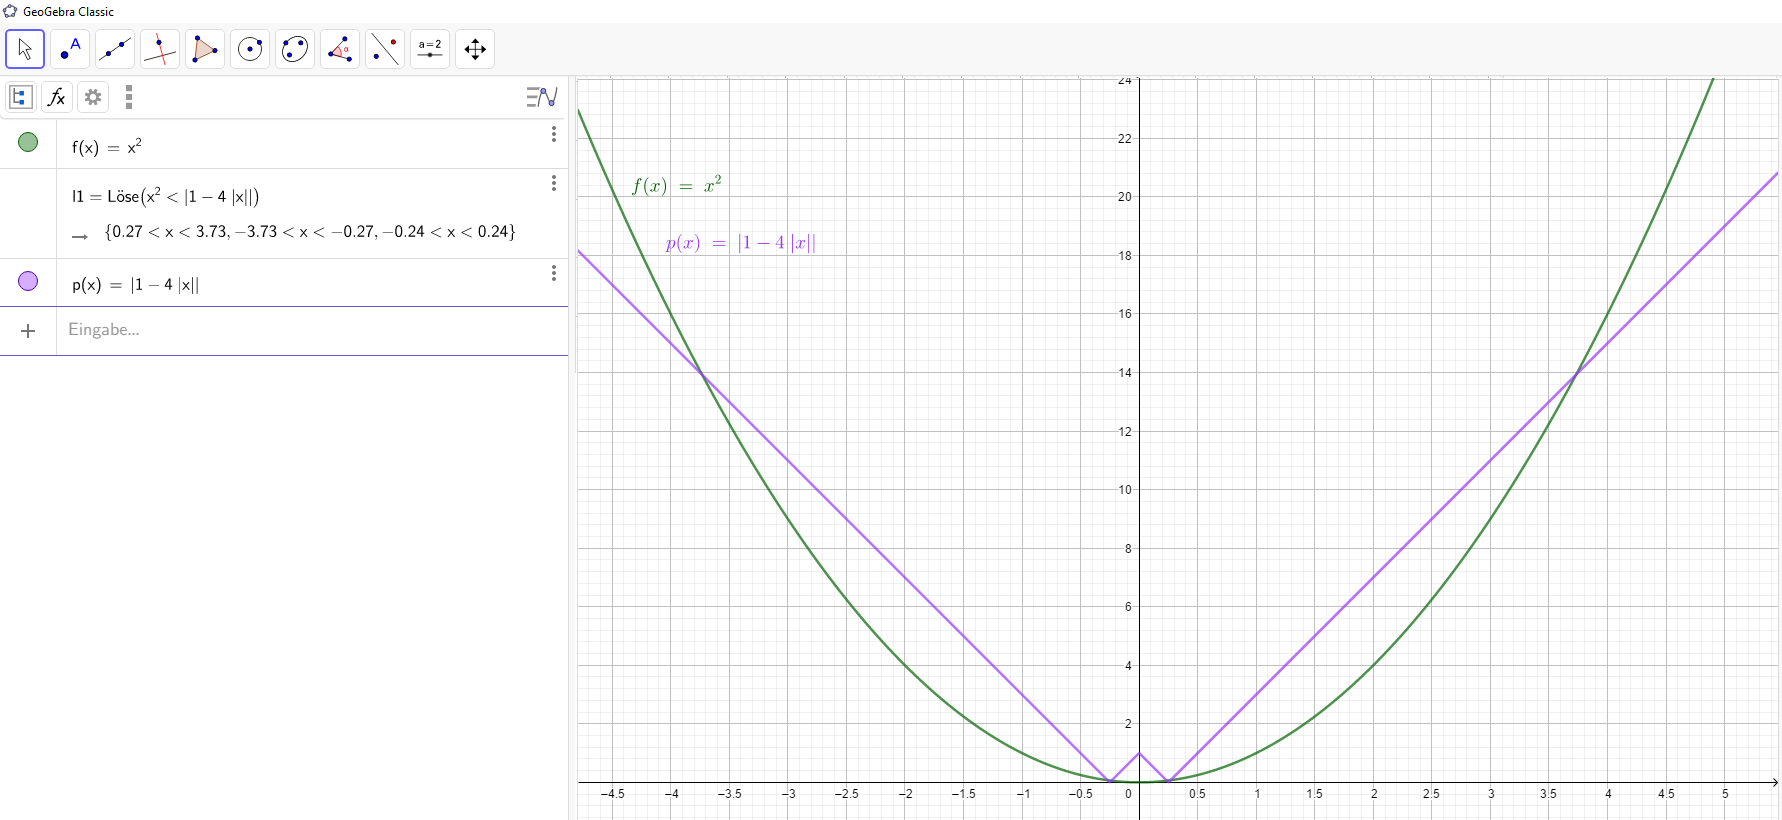
\includegraphics[width=\textwidth]{../Mathematik_2/Bilder/zahlenreihen_konvergenz_funktionsgraphen.png}
			\end{center}
		\item[(b)] F�r jedes \(x\in\mathbb L\) konvergiert die Reihe mit \(s(x) = \displaystyle{\frac{x^2}{1-x}}\)\,.
	\end{itemize}
\end{exercisebox}

